\section{Introduction}

The general communication channel is equivalent to a conditional probability distribution function (pdf). The pdf $p(\mathbf{x}|\mathbf{y})$ takes into account the potentially random channel though which the transmitted information $\mathbf{x}$ passes to reach a receiver as the information $\mathbf{y}$ \cite[Ch.~7]{cover2012elements}. Selecting the most probable transmitted information sequence based on the received information sequence is known as maximum a posteriori (MAP) sequence estimation. In general, sub-optimal solutions to this estimation problem do not require perfect knowledge of the pdf $p(\mathbf{x}|\mathbf{y})$ and may be used when the true $p(\mathbf{x}|\mathbf{y})$ is unknown or impractical to obtain.

\par
Some communication contexts, including wireless, have successfully used "pilot" symbol-streams to estimate the pdf $p(\mathbf{x}|\mathbf{y})$ \cite{van1995channel}. The receiver is informed of a specific symbol sequence prior to receiving that same sequence sent through the channel. The receiver may then compare the received signal with the known ground truth to estimate the channel $p(\mathbf{x}|\mathbf{y})$.
The use of pilot sequences relies on a pre-selected channel model whose parameters are determined using the pilot sequence. For example, if the channel is assumed to be a noiseless, linear and time-invariant (LTI) system, the pilot sequences may be used to find the exact impulse response of the channel, as will be seen in Section \ref{LMMSE}. In some cases, however, a precise channel model may not be available. This work investigates the parameterization of a very general channel model for $p(\mathbf{x}|\mathbf{y})$ using a neural network. In \cite{shlezinger2019viterbinet} and \cite{shlezinger2020datadriven}, a neural network-based estimation of the channel is shown to be an effective method for detection with incomplete channel information for LTI channels.
 Extending on this, we look to estimate $p(\mathbf{x}|\mathbf{y})$ for channels in the molecular communication domain.
 We also look to exploit any redundancy in the pdf $p(\mathbf{x}|\mathbf{y})$ in order to reduce the complexity of the resulting detection algorithm.
\par
Molecular communication channels can be difficult to characterize due to non-linear and random components of the channel that may be either independent or dependent on the transmitted information. As a result, molecular communication channels are good candidates for testing this estimation technique. For a thorough review and mathematical formulation of molecular communication channels and their applications, see \cite{jamali2019channel}. 

\par

\section{System Model}

A system model is now developed as a consistent communication framework to be used in the remainder.
\par
We consider a point-to-point communication system as in Figure \ref{fig:model} with a transmitter sending a sequence of information $\mathbf{x}$ over a channel. At the receiver, the sequence  $\mathbf{y}$ is detected. 
The individual elements of $\mathbf{x}$ are chosen from a finite symbol alphabet $\textit{\cal{A}}$ such that the kth symbol in $\mathbf{x}$, $x[\text{k}]$, is selected from  $\textit{\cal{A}}$.

\begin{figure}[H]
\begin{tikzpicture}[node distance=2cm]
\node (transmitter) [process] {Transmitter: $\mathbf{x}$};
\node (channel) [process, right = of transmitter] {Channel};
\node (receiver) [process, right = of channel] {Receiver: $\mathbf{y}$};
\draw [arrow] (transmitter) -- (channel);
\draw [arrow] (channel) -- (receiver);
\end{tikzpicture}
\caption{The point-to-point communication system.}
\label{fig:model}
\end{figure}

The components of the vector $\mathbf{y}$ are given by
\begin{equation*}
y[\text{k}] = f_{\text{k}}(\mathbf{x}) + n[\text{k}],
\end{equation*}
with independent $n[\text{k}]\sim \mathcal{N}(0,1).$
Allowing for $f_{\text{k}}(\cdot)$ to be a general and potentially random function for time index k, each received symbol $y[\text{k}]$ is potentially a function of all transmitted information $\mathbf{x}$. By assuming all $n[\text{k}]$ to be independent, an orthogonal filtering at the receiver of the modulated information $\mathbf{x}$ is implied. 

We define the signal to noise ratio (SNR) at the receiver as

\begin{equation*}
\text{SNR} = \frac{E\{|x[\text{k}]|^2\}}{\{|n[\text{k}]|^2\}}.
\end{equation*}
\par
We now consider specific cases for the function $f_{\text{k}}(\cdot)$. \par
In the first communication channel considered, each $y[\text{k}]$ is a causal, linear, and time-invariant (LTI) combination of the transmitted sequence $[x[\text{k}], x[\text{k}-1]... x[\text{k}-\text{L}+1]]$ weighted by coefficients $[a[0], a[1].. . [\text{L}-1]]$ (the channel impulse response). 
\begin{equation}\label{lti_channel}
y[k] = \sum_{\mathrm{\text{l}=0}}^{\mathrm{\text{L}-1}} a[\text{l}]x[\text{k}-\text{l}]+ n[\text{k}].
\end{equation}
In order to preserve the defined SNR, we consider the case in which the impulse response vector is unit normalized such that $\|\mathbf{a}\|^2 =1 $. This is also enforced in simulations discussed in Section \ref{real_results}.
\par
We also consider the case in which the output from an arbitrary communication channel is the input to a quantizer defined by 
\[\text{quant}(x) = 
\begin{cases}
\text{sign}(x)\text{floor}\left(\frac{|x|}{\text{step-size}}\right)& \text{lower saturation level} \leq x \leq \text{upper saturation level}\\
\text{upper saturation level} & x \geq \text{upper saturation level}\\
\text{lower saturation level} & x \leq \text{lower saturation level}
\end{cases}
\]
 and  
 \begin{equation*}
  \text{step-size} =\text{floor}\left(\frac{|\text{upper saturation level}- \text{lower saturation level}|}{\text{\#quantization levels}}\right)
 \end{equation*} for a given number of quantization levels with an upper and lower saturation level. A quantization function with 11 quantization levels and lower/upper saturation levels -0.5/+0.5 respectively is shown in Figure \ref{fig:Quantized Overlay}. 
  \begin{figure}[H]
\centering
	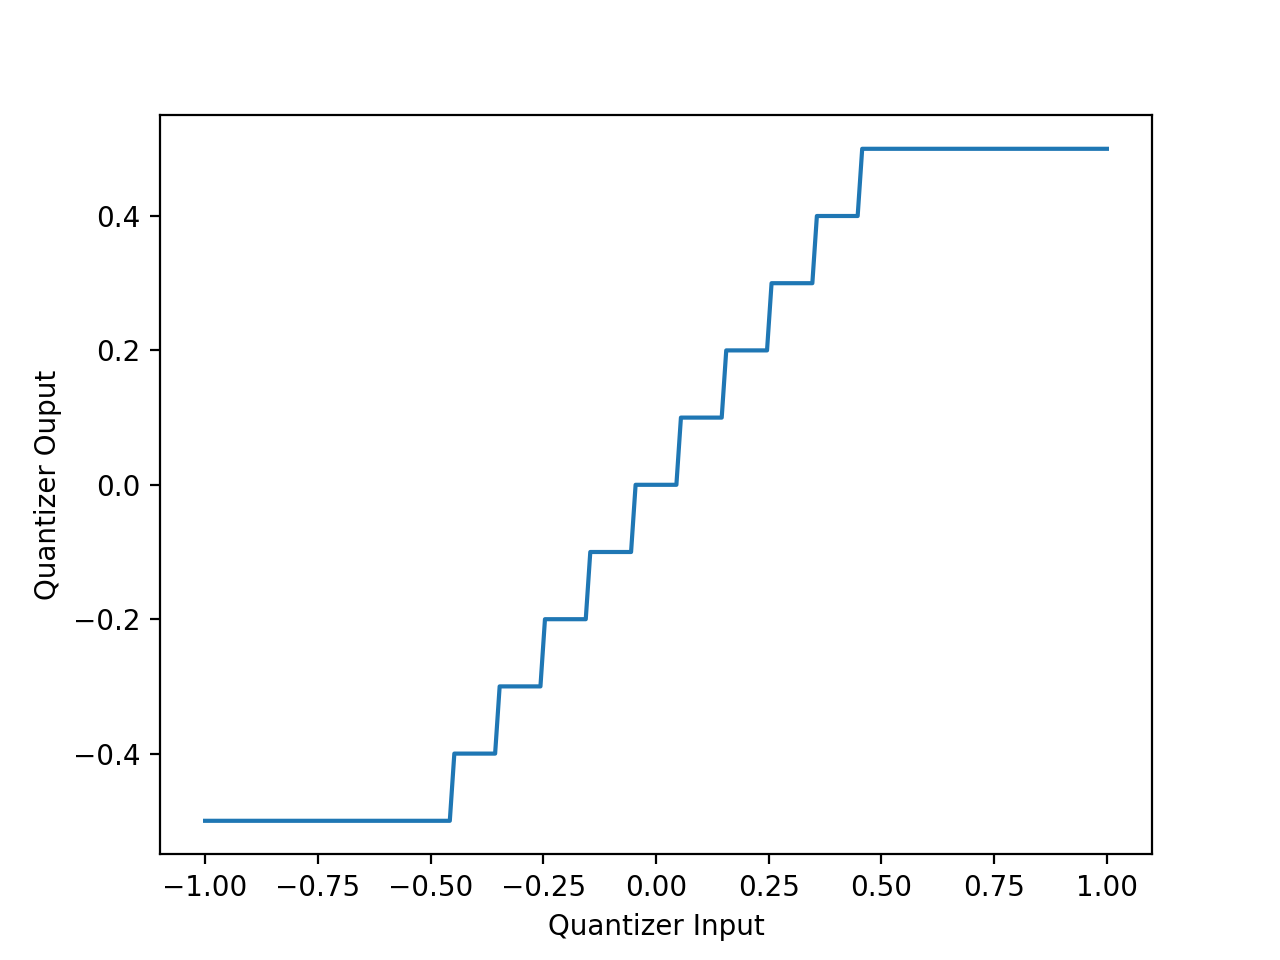
\includegraphics[width=10cm,height = 10cm]{system_model/quantizer_good}
			  \caption{A Quantization function with with 11 levels of quantization, lower saturation level -0.5 and upper saturation level 0.5. }
	  \label{fig:Quantized Overlay}
\end{figure}
 
After quantization the received signal is then given by 
\begin{equation}\label{lti_quantized_channel}
y[\text{k}] = \text{quant}(f_{\text{k}}(\mathbf{x}) + n[\text{k}]).
\end{equation}

 


 
\section{Background}
The following section first introduces the optimization problem used in the remainder of this work. An efficient implementation for solving the optimization problem is then introduced. With this foundation in place, the data-driven, neural network-based estimator is then incorporated into the optimization algorithm to give a neural network-based equalizer. 
Extending on the neural network-based equalizer, a method to further reduce the algorithm complexity is then considered. Last, a linear equalizer is derived to be used as a reference in the simulation results. 
\subsection{The Viterbi Algorithm}
Rather than considering only the transmitted symbols $\mathbf{x}$ for the MAP problem described above, we consider instead a system in which a sequence $\mathbf{y}$ is received from a channel which may take on a set of states $\{s_1, s_2... \;s_{\text{L}}\} = \textit{\cal{S}}$. With knowledge of the potential states $\{s_1, s_2... s_{\text{L}}\}$ but not of the sequence of realized states, $[s[1], s[2]... \; s[\text{N}]] \in \;\textit{\cal{S}}^N $, corresponding to the observed sequence, $[y[1], y[2]... \; y[\text{N}]]$, the MAP problem is formalized as

\begin{equation*}
\underset{\mathbf{s}\in\textit{\cal{S}}^N}{\text{argmax}} \; p(\mathbf{s}|\mathbf{y}).
\end{equation*} 

Using Bayes' theorem, gives
\begin{equation*}
p(\mathbf{s}|\mathbf{y}) = 
\frac
{p(\mathbf{y}|\mathbf{s})p(\mathbf{s})}
{p(\mathbf{y})}.
\end{equation*} 
The term $p(\mathbf{y})$ is independent of $\mathbf{s}$ and is removed without effect. The resulting optimization problem
\begin{equation}\label{opt_problem}
\underset{\mathbf{s}\in\textit{\cal{S}}^N}{\text{argmax}}\; p(\mathbf{y}|\mathbf{s})p(\mathbf{s})
\end{equation}
will be used in the remainder.
Noting that the size of the search space $|\textit{\cal{S}}^N|$ grows exponentially in $N$, the length of the received sequence, a method for reducing the search complexity is now introduced. 
\par
For the LTI communication channel with impulse response length L, defined by equation \eqref{lti_channel}, each state $s_i \in \{s_1, s_2... \; s_{\text{L}}\}$ represents a transmitted sequence $[x[\mathrm{i-L+1}]...\;x[\mathrm{i}]]$, implying a specific transmit sequence memory. Therefore, a state sequence $\mathbf{s}$ is only possible if the states do not have contradicting channel memory. This can be formalized by noticing that for the LTI system, the sequence of states satisfies the property  
\begin{equation*}
p(\mathbf{s}) = p(s[\text{N}]|s[\text{N-1}]) p(s[\text{N-1}]|s[\text{N-2}])... \;p(s[\text{2}]|s[\text{1}])p(s[\text{1}]),
\end{equation*}
or equivalently, that the channel state sequence satisfies the Markov property given by 
\begin{equation*}
p(s[\text{k}]|\left[s[\mathrm{k-1}]... \;s[\mathrm{1}]\right]) = p(s[\text{k}]|s[\text{k-1}]).
\end{equation*}
For this channel, the MAP sequence estimation is given by
\begin{gather*}
\underset{\mathbf{s}\in\textit{\cal{S}}^N}{\text{argmax}} \; p(\mathbf{y}|\mathbf{s})p(\mathbf{s})=
\underset{\mathbf{s}\in\textit{\cal{S}}^N}{\text{argmin}} \; \sum_{\mathrm{k=1}}^{\mathrm{N}} -\text{log}(p(y[\mathrm{k}]|s[\mathrm{k}]) p(s[\mathrm{k}]|s[\mathrm{k-1}]))=\\
\underset{\mathbf{x}\in\textit{\cal{A}}^N}{\text{argmin}} \; \sum_{\mathrm{k=1}}^{\mathrm{N}} -\text{log}(p(y[\mathrm{k}]|\left[x[\mathrm{k-L+1}]...x[\mathrm{k}]\right]) p(\left[x[\mathrm{k-L+1}]...\;x[\mathrm{k}]\right]|\left[x[\mathrm{k-L}]...\;x[\mathrm{k-1}]\right])),
\end{gather*}
in which individual terms of the sums are statistically independent. The optimization problem is now equivalently
  represented by a graph with the L states $\{s_1, s_2... \;s_{\text{L}}\}$ repeated N times and all states in time k, $s_{\text{i}}[\text{k}]$ for $ i = 1... \;L$, connected to all states in time k$+1$, $s_{\text{i}}[\text{k+1}]$ for $ i = 1... \;L$,
   with an edge weighted by
\begin{equation*}
-\text{log}(p(y[\text{k}+1]|s_{\text{i}}[\text{k+1}])p(s_{\text{i}}[\text{k+1}]|s_{\text{j}}[\text{k}])).
\end{equation*}   
This is illustrated in the following example. 
   \par
   We consider the communication system with $\textit{\cal{A}}=\{0, 1\}$ and received symbols 
   \begin{equation*}
y[\text{k}] =  a[\text{0}]x[\text{k}] + a[\text{1}]x[\text{k}-1] + n[\text{k}].
\end{equation*}

The resulting state graph (or trellis) is depicted in Figure \ref{fig:trellis}. 
\begin{figure}[H]
\begin{center}
\begin{tikzpicture}[]
% 1st column
\node               at (-1.5,5) {$s_1=00$};
\node               at (-1.5,4) {$s_2=01$};
\node               at (-1.5,3) {$s_3=10$};
\node               at (-1.5,2) {$s_4=11$};
\node[mainstate] (s1_1) at (0,5) {$s_1$};
\node[state] (s2_1) at (0,4) {$s_2$};
\node[state] (s3_1) at (0,3) {$s_3$};
\node[state] (s4_1) at (0,2) {$s_4$};
%\node at (0,1) {Node1};
% 2nd column
\node[mainstate] (s1_2) at (2,5) {$s_1$}
    edge[mainedge] (s1_1);
\node[mainstate] (s2_2) at (2,4) {$s_2$}
     edge[lightedge] (s1_1);

\node[state] (s3_2) at (2,3) {$s_3$};

\node[state] (s4_2) at (2,2) {$s_4$};

%\node at (2,1) {Node2};
% 3rd column
%\node               at (4,6) {$t=2$};
\node[mainstate] (s1_3) at (4,5) {$s_1$}
    edge[mainedge]  (s1_2);

\node[mainstate] (s2_3) at (4,4) {$s_2$}
    edge[lightedge] (s1_2);

\node[mainstate] (s3_3) at (4,3) {$s_3$}
    edge[mainedge] (s2_2);    
\node[mainstate] (s4_3) at (4,2) {$s_4$}
    edge[lightedge] (s2_2);
%\node at (4,1) {Node3};
% 4th column
%\node               at (6,6) {$t=3$};
\node[mainstate] (s1_4) at (6,5) {$s_1$}
    edge[mainedge]  (s1_3)
    edge[mainedge]  (s3_3);
\node[mainstate] (s2_4) at (6,4) {$s_2$}
    edge[lightedge] (s1_3)
    edge[lightedge] (s3_3);
\node[mainstate] (s3_4) at (6,3) {$s_3$}
    edge[mainedge] (s2_3)
    edge[mainedge] (s4_3);
\node[mainstate] (s4_4) at (6,2) {$s_4$}
    edge[lightedge] (s2_3)
    edge[lightedge] (s4_3);
%\node at (6,1) {Node4};

\end{tikzpicture}
	\end{center}
	\caption{MLSE decoding for $\mathcal{A}=\{0,1\}$ and $L=2$. Each state $s_1 ... \; s_4$ represents a possible transmit symbol sequence
	$\left[x[\mathrm{i-L+1}]...x[\mathrm{i}]\right]$.}
	\label{fig:trellis}
\end{figure}
Assuming equiprobable 
$x[\text{k}] \in \textit{\cal{A}}$, the value of $p(s_{\text{j}}[\text{k+1}]|s_{\text{i}}[\text{k}])$ for connected states $s_{\text{j}}[\text{k+1}]$ and $s_{\text{i}}[\text{k}]$ is  0, if the channel memory represented by $s_{\text{j}}[\text{k+1}]$ and $s_{\text{i}}[\text{k}]$ contradicts, and otherwise $p(s_{\text{j}}[\text{k+1}]|s_{\text{i}}[\text{k}])$  is some constant c ($0<$ c $\leq1$). For clarity, all edges for which $p(s_{\text{j}}[\text{k+1}]|s_{\text{i}}[\text{k}])=0$ have been removed in Figure \ref{fig:trellis}. The solution to Problem \ref{opt_problem} corresponds to the minimum cost path through all N sets of states, which can be found using the Viteribi algorithm. 
\\

    \noindent\rule[16pt]{\textwidth}{0.6pt}
	Viterbi Algorithm

    \noindent\rule[10pt]{\textwidth}{0.4pt}
    {\footnotesize
    \begin{tabbing}
        {\textbf{given}} $p(y[\text{k}]|s_{\text{i}}[\text{k}])$, $p(s_{\text{i}}[\text{k+1}]|s_{\text{j}}[\text{k}]) \; \forall  \; \text{k} \in {1...\;N}$, $ \forall \; \text{i} \in {1...\;L}$ and $ \forall \; \text{j} \in {1...\;L}$.\\
        {\textbf{initialize}} $\text{cost}_{\text{i}}[0]=0, \; \forall \; \text{i} \in {1...\;L}$
         \\*[\smallskipamount]
        {\textbf{for}  $\text{k} = 1... \; N $} \\
         \qquad \= {\textbf{for} $\text{i} = 1... \; L$}\\
        \qquad \qquad \= \textbf{Let} $\text{cost}_{\text{i}}[\text{k}] = \underset{\text{j} \in \{1... \; L\}} {\text{argmin}}\left( \text{cost}_{\text{j}}[\text{k-1}]
        -\text{log}(p(y[\text{k}]|s_{\text{i}}[\text{k}])p(s_{\text{i}}[\text{k}]|s_{\text{j}}[\text{k-1}]))
        \right)$ \\
        {\textbf{ return}} the sequence of states, $\mathbf{s}$, corresponding to the path of $\underset{\text{i} \in \{1... \; L\}} {\text{argmin}} \; \text{cost}_{i}[\text{N}] $
    \end{tabbing}}
    \noindent\rule[10pt]{\textwidth}{0.4pt}





Note that the Viterbi algorithm is \emph{linearly} complex in the length of the sequence $\mathbf{s}$ ($N$ in the algorithm above) but \emph{exponentially} complex in the number of channel states $|\textit{\cal{S}}|$ at each time index. 
\par
The above model allows channels whose state is based upon transmitted symbols to be represented using a trellis, such as the LTI channel. This graph-based model can also generalize to represent channels with certain kinds randomness that is \emph{independent} of the transmitted symbols. In this case, the model is constrained to channels whose state sequence satisfies the Markov property.
\par
This model can also represent the case in which a channel state, $s_{\text{i}}[k]$, does not uniquely identify a symbol that was transmitted in the corresponding time index, $x[\text{k}]$. While this case requires additional tools to ultimately arrive at a unique transmit sequence $\mathbf{x}$, it may also reduce the complexity of the corresponding Viterbi algorithm. This case will be considered further in Section \ref{reduced_viterbi}.
\par
Before moving on, an example is posed for which the states of this framework represent more than just the transmitted sequence memory. We allow for the  receiver from equation \ref{lti_channel} to have a noise floor such that 
\begin{equation}\label{lti_channel_floor}
y[\text{k}] = \sum_{\mathrm{\text{l}=0}}^{\mathrm{\text{L}-1}} a[\text{l}]x[\text{k}-\text{l}]+ n[\text{k}]+ b[\text{k}](\text{noise floor})
\end{equation}
still with $n[\text{k}]\sim \mathcal{N}(0,1)$ and the Bernoulli random variable $b[\text{k}]$ describing a fluctuating noise floor at the receiver. In this case, the states from the original LTI system are extended to indicate the noise floor state for the time index of each received symbol $y[\text{k}]$. When $b[\text{k}]$ is a Bernoulli random variable, this results in doubling the number of states in each step of the Viterbi algorithm. 

In the remainder of this background, we consider the case in which the  channel state is determined entirely by $\left[x[\mathrm{i-L+1}]...x[\mathrm{i}]\right]$.

\subsection{ViterbiNet}

Despite the complexity reduction of the Viterbi Algorithm for MAP detection, weighting the edges of the trellis requires knowledge of the channel probability distribution $p(y[\mathrm{k}]|s_{\text{i}}[\text{k}])$. Rather than estimate this function directly, we use Bayes' theorem and instead estimate the individual terms of
\begin{equation*}
p(y[\mathrm{k}]|s_{\text{i}}[\text{k}]) = 
\frac
{p(s_{\text{i}}[\text{k}]|y[\mathrm{k}])p(y[\mathrm{k}])}
{p(s_{\text{i}}[\text{k}])}.
\end{equation*}

\begin{itemize}
\item $p(s_{\text{i}}[\text{k}]|y[\mathrm{k}])$: 
For a channel with finite states $\{s_1, s_2,...\; s_{\text{L}}\}$, this probability mass function can be estimated using a neural network for classification. Each training data pair includes a single received pilot symbol $y[\text{k}]$ (the network input ) and the probability of being in each state
$s_{\text{i}}[\text{k}] \sim \left[x[\mathrm{i-L+1}]...x[\mathrm{i}]\right]$ (the network output). The true state is known for pilot symbols. By using a network architecture with a number of outputs corresponding to the number of channel states, the trained network will output the desired $p(s_{\text{i}}[\text{k}]|y[\text{k}])$ for all $s_{\mathrm{i}} \in \textit{\cal{S}}$. Figure \ref{nn} depicts the neural network for a channel with four states. The shown network has a total of 20 weighted edges (model parameters) to be optimized during training. For a detailed review of classification using neural networks, see \cite[Ch.~5]{Goodfellow-et-al-2016}.

	\begin{figure}[H]
	\centering
		\begin{neuralnetwork}[height=4.5, nodespacing=20mm, layerspacing=26mm]
		\newcommand{\x}[2]{$y[\text{k}]$}
		\newcommand{\y}[2]{$p(s_{#2}[\text{k}]|y[\text{k}])$}
		\newcommand{\hfirst}[2]{ $h^{(1)}_#2$}
		\newcommand{\hsecond}[2]{ $h^{(2)}_#2$}
		\newcommand{\hthird}[2]{$h^{(3)}_#2$}
		\newcommand{\hfourth}[2]{$h^{(4)}_#2$}
		\inputlayer[count=1, bias=false, title=Received\\, text=\x]
		\hiddenlayer[count=2, bias=false, title=\\, text=\hthird] \linklayers
		\hiddenlayer[count=3, bias=false, title=\\, text=\hfourth] \linklayers
		\outputlayer[count=4, title=States\\, text=\y] \linklayers
	    \end{neuralnetwork}
	    	  	  \caption{A fully-connected, feed-forward neural network architecture for classification of received symbols $y[\text{k}]$ into four channel states.}
\label{nn}
	\end{figure}

\item $p(y[\mathrm{k}]) = \sum_{s_{\mathrm{i}} \in \textit{$\textit{\cal{S}}$}}p(s_{\mathrm{i}},y[\mathrm{i}])$: This term is found by marginalizing the joint probability of channel state $s_{\mathrm{i}}[\mathrm{k}]$ and received signal $y[\mathrm{k}]$ over all channel states in $\textit{\cal{S}}$. As $p(y[\mathrm{k}])$ is constant over all states in a given step of the Viterbi algorithm, it may be interpreted as a weighting factor for the cost of received symbol $y[\mathrm{k}]$ relative to other symbols $y[\mathrm{j}], \; j\neq k$. For example, if $y[\mathrm{k}]$ is received under improbable noise and channel state, this term would reduce the overall impact of $y[\mathrm{k}]$ on the final path chosen through the graph. In the case of equiprobable channel states without receiver noise, $p(y[\mathrm{k}])$ would be constant and have no impact on the chosen path.
\par
This probability distribution function can be estimated using a so-called mixture model. This requires pre-selecting the number of considered channel states and a parameterized model for the receiver noise. The Expectation Maximization algorithm, detailed in \cite{ng2000cs229}, along with a set of channel output data, can be used to optimize the parameters of this model. Unlike parameterizing the neural network, this algorithm does not require labeled data from pilot sequences. An example in which the mean of 16 Gaussian sources calculated for the output of an LTI channel with 16 states (Gaussian sources) is shown in Figure \ref{fig:mm}. It is seen in Figure \ref{fig:mm} that some of the sources result in closely overlapping output observed at the receiver. 
%\\
%
%    \noindent\rule[16pt]{\textwidth}{0.6pt}
%	Expectation Maximization Algorithm for Gaussian Mixture Model: (TODO Discuss how much derivation is needed here)
%
%    \noindent\rule[10pt]{\textwidth}{0.4pt}
%    {\footnotesize
%    \begin{tabbing}
%        {\bf given} $p(y_{\mathrm{i}}|x_{\mathrm{i-L+1}}^{\mathrm{i}}) \; \forall i \in {1..N}$ . \\*[\smallskipamount]
%        {\bf for $i = 1..N $} \\
%         \qquad \= {\bf for each state $s$ at time $i$}\\
%        \qquad \qquad \= 1.\ Let $\textit{survivor cost}_{s}  += \text{min}\{\text{incoming transition costs}\}$ \\
%%        \> 2.\ {\bf break if} $f(z) \leq \hat{f}_{\lambda}(z, x^{k})$. \\
%%        \> 3.\ Update $\lambda := \beta \lambda$. \\*[\smallskipamount]
%        {\bf return} Symbols corresponding to path of $\underset{s}{\text{argmin}} \; \textit{survivor cost}_{s} $
%    \end{tabbing}}
%    \noindent\rule[10pt]{\textwidth}{0.4pt}


%picture of MM
%	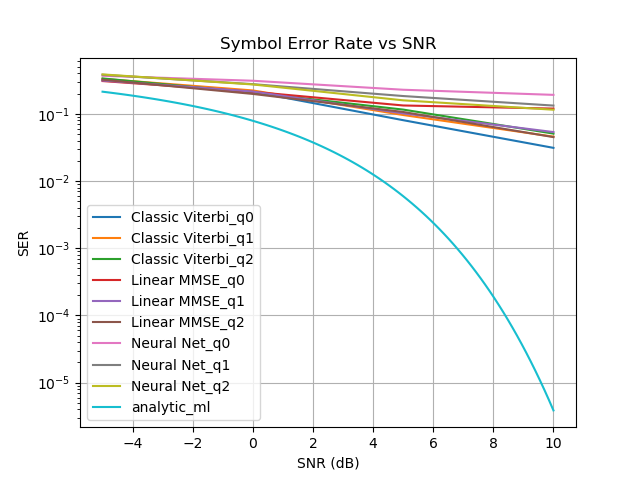
\includegraphics[width=\textwidth,height = 7cm]{results/quant_standard}

\begin{figure}[H]
\centering
	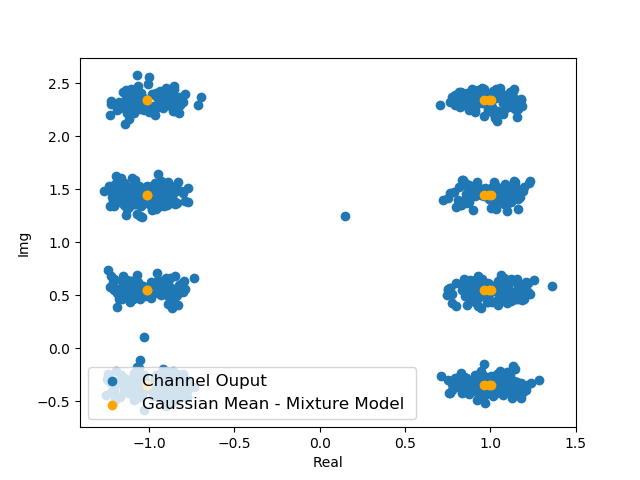
\includegraphics[width=\textwidth,height = 10cm]{system_model/mixture_model}
	  	  \caption{A mixture of complex, Gaussian sources and the averages of the Gaussian sources predicted using the Expectation Maximization algorithm}
	  \label{fig:mm}
\end{figure}

\item $p(s[\text{k}])$: For the case in which channel states are equiprobable, such as when $s_{\text{k}}$ corresponds to $\left[x[\mathrm{i-L+1}]...x[\mathrm{i}]\right] \in \textit{\cal{A}}^{\mathrm{L}}$, this term will not influence the final path.

\end{itemize}

Combining these terms and their impact on the original $p(y[\mathrm{k}]|s_{\text{i}}[\text{k}])$, each edge weight used in the Viterbi algorithm essentially gives the probability of simultaneously arriving at a state $s_{\text{i}}[\text{k}]$ conditioned on the previous state $s_{\text{i}}[\text{k-1}]$ and the probability of receiving $y[\mathrm{k}]$ based on the channel and noise. 

We now consider how a channel might be represented using the minimum number of states.


\subsection{A Reduced-State ViterbiNet}\label{reduced_viterbi}
While the Viterbi Algorithm complexity scales exponentially with the number of states possible in each step of the algorithm, in some cases this complexity can be reduced without significant loss of detection performance. One well-established method to achieve this is by prefiltering the incoming signal so as have a minimum-phase representation of the channel, as in \cite{gerstacker2000efficient}. Such methods are, however, dependent upon an estimate of the channel, which  implies an assumed underlying channel model. In this section, we consider a method for complexity reduction without prefiltering the estimated channel.

%There are two things to note here, first, this prefiltering works for LTI channels but may not be possible for channels with non-linearities (such as molecular communication channels). Also note that even this minimum phase representation of the channel still has redundancy that could be reduced using this method. Finally, this prefiltering assumes some sort of estimate and model of the channel that we are trying to abstract from in this work for generality. 


The following, illustrative example proposes a channel whose states, as seen by the receiver, contains redundancy. A method for reducing the number of states based on this observed redundancy is then considered. 

The received signal from an LTI communication channel
\begin{equation*}
y[k] = \sum_{\mathrm{l=0}}^{\mathrm{L-1}} a[l]x[k-l] + n[k], \; n[k]  \sim \mathcal{N}(0,1),
\end{equation*}
with  $\textit{\cal{A}}=\{-1, 1\}$, $n[k]  \sim \mathcal{N}(0,1)$ and 
channel impulse response $\mathbf{a} = [a[1]...a[5]]=[1, 0, .2, .2, .4]$ ($\|\mathbf{a}\|^2_2 = 1$),  is shown in Figure \ref{fig:redundant_channel}. Desipite having channel memory L $=5$, there are fewer than the potential $|\textit{\cal{A}}^5| =2^5$ clusters of received signals. This is due to the redundancy in the channel.  As one of the channel taps is 0, this will have no impact on the output seen at the receiver and thus 16 of the potential 32 states are not observed at the receiver. Additionally, because $\left[a[2],a[3]\right] = \left[0.2, 0.2 \right] $, the cases in which  $\left[x[k-2],x[k-3]\right] = [-1,1]$ and $\left[x[k-2],x[k-3]\right] = [1,-1]$, will map to the same output as seen by the receiver. 

%\begin{figure}[H]
%\centering
%	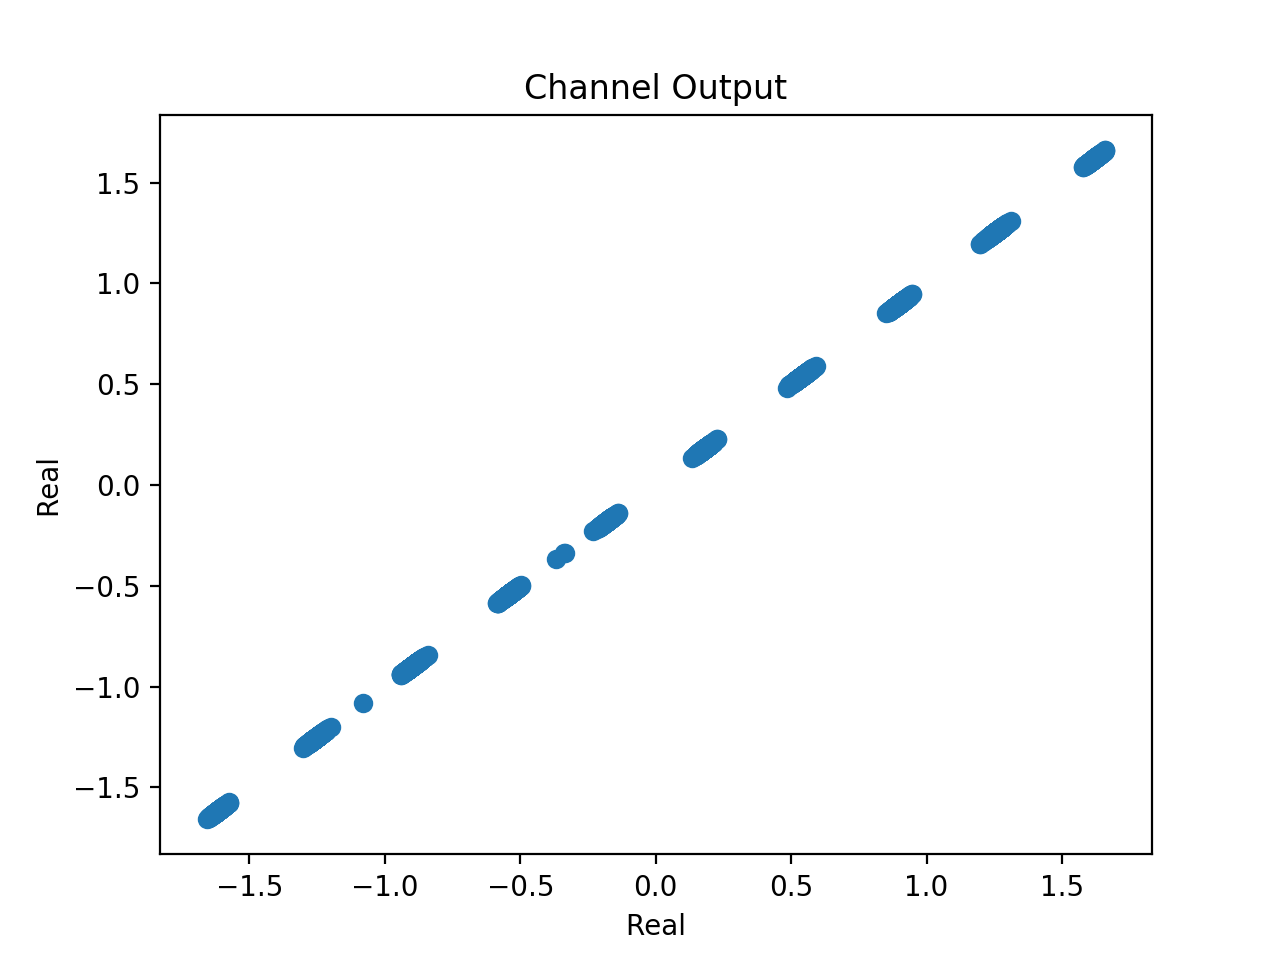
\includegraphics[width=10cm,height = 10cm]{system_model/channel_output}
%	  \label{fig:redundant_channel}
%	  	  \caption{LTI channel with state redundancy with high SNR}
%\end{figure}

\par
One data-driven approach to exploiting state redundancy is to cluster the observed states (receiver output) into a set of $k<|\textit{\cal{S}}|$ clusters using training data. The k-Means algorithm is proposed as one such clustering method.
\\

    \noindent\rule[16pt]{\textwidth}{0.6pt}
k-Means Clustering Algorithm: A method for unsupervised classification. 
    \noindent\rule[10pt]{\textwidth}{0.4pt}
    {\footnotesize
    \begin{tabbing}
        {\textbf {given}} a set of N training points $x[{\mathrm{i}}], \;\mathrm{i} = [1...\;N]$.\\
    {\textbf {select}} random, initial locations of centroids $L_c$, for $c = [1...\; \text{K}]$.\\
        {\textbf{for} a chosen number of iterations}:\\
         \qquad \= {\textbf {for} training data point $x[{\mathrm{i}}], \;\mathrm{i} = [1... \;N]$}:\\
        \qquad \qquad \= 1.\ Label $x[\text[i]]$ with the index, c, of the closest centroid using $\|x[{\mathrm{i}}]- \text{L}_c\|^2_2$. \\
        \qquad \= {\textbf {for} centroid $L_c$,  $c = [1...\; \text{K}]$}:\\
                \qquad \qquad \= 1.\ Move $L_{\mathrm{c}}$ to the average location of all training points $x[\text[i]]$ with label c.\\*[\smallskipamount]
        {\textbf{return}} centroid locations, $L_c$, for $c = [1...\; \text{K}]$.
    \end{tabbing}}
%    Note that this algorithm implements a generally non-convex optimization problem and thus the initial locations chosen for $L_c$ for $c = [1...\; \text{K}]$ may impact the final locations of each $L_c$.
    \noindent\rule[10pt]{\textwidth}{0.4pt}
    
With a pilot sequence training set, a mapping of the original states into the new $k<|\textit{\cal{S}}|$ states is performed by finding which of the $k$ new states (clusters) includes the most trainings examples from the known, original state $s_{\text{i}}$ for i = $[1...\; L]$. The Viterbi algorithm can then be performed to find the MAP state sequence $\mathbf{s}$. 
An important implementation consideration for this clustering approach is now discussed. 
\par
If the channel has memory $\text{L}>1$, some of the channels states represent different transmit sequence history. If states with contradicting transmission history are clustered together, the choice for the transmitted symbol at the index of contradiction is unclear. To accommodate this scenario, a majority rule decision is made, based on the final state path chosen by the Viterbi algorithm. During the clustering procedure, the fraction of training samples from each original state placed into each reduced state is recorded to give the likelihood of each symbol in the transmitted symbol memory for each of the reduced states. After finding the MAP state sequence $\mathbf{s}$, the probability of each symbol in $\textit{\cal{A}}$ is found for each time index. The most likely symbol is chosen in order to find a transmitted sequence estimate $\mathbf{x}$. 
\par
The performance of the proposed system will depend on the whether or not the number of clusters, k, corresponds to the true number of states observed by the receiver. If k is much smaller than the number of observed states, the performance will suffer. Again considering the LTI channel with AWGN, if k is smaller than the observed number of clusters at the receiver, the equalization will be disregarding a component of the channel memory, and as a result, may perform poorly.
\par
Before discussing the results of simulations using the neural network-based equalization schemes, a fundamental, low-complexity equalization scheme is introduced.

\subsection{Equalization Benchmark}\label{LMMSE}
The Linear Minimum Mean-Squared Error (LMMSE) equalizer derived in the following is used to provide a linear equalization reference to the proposed neural network-based equalization which is non-linear.
\par
Given an estimate of channel memory length L, the convex and continuously differentiable optimization problem 

\begin{equation*}\label{mmse}
\underset{\mathbf{\mathbf{h}} \in \mathcal{C}^{\text{L}}}{\text{argmin}} \;
 E[\|x-\mathbf{h}^T\mathbf{y}\|^2],
\end{equation*}\
minimizes the squared difference of the linearly detected symbol $\hat{x}= \mathbf{h}^T\mathbf{y}$ and true symbol $x$.
Using
\begin{equation*}\label{mmse}
\frac{\partial  E[\|x-\mathbf{h}^T\mathbf{y}\|^2]}{\partial \mathbf{h} } = 0
\end{equation*}
the optimal LMMSE equalizer is \cite{proakis1988introduction}
\begin{equation*}\label{mmse}
\mathbf{h} = E[\mathbf{R}_{yy}]^{-1}E[\mathbf{r}_{yx}].
\end{equation*}
$E[\mathbf{R}_{yy}]$ and $E[\mathbf{r}_{yx}]$ are estimated by
\begin{equation*}\label{mmse}
 E[\mathbf{R}_{yy}]= \frac{1}{\mathrm{N}}\sum_{\mathrm{i=1}}^{\mathrm{N}}
\mathbf{y^{\text{i}}_{\text{i-L+1}}}\mathbf{y^{\text{i}}_{\text{i-L+1}}}^H
 \end{equation*}
 and
\begin{equation*}\label{mmse}
E[\mathbf{r}_{yx}]= \frac{1}{\mathrm{N}}\sum_{\mathrm{i=1}}^{\mathrm{N}}
\mathbf{y^{\text{i}}_{\text{i-L+1}}}x_{\text{i}},
 \end{equation*}
 using the same training data as the neural network and mixture model. 
 
\par
One interesting note to make in comparing this equalizer with the neural network-based equalizer is the amount of training data needed. In the case of the noiseless LTI system, a linear estimator for the channel requires only L training examples to form a deterministic system of equations and learn the channel perfectly. In contrast the neural network will generally have many edge weights and would therefore require more training data. The need for a larger training data set, however, comes with the potential to learn more complicated channels with the neural network than with the LMMSE equalizer.
 
\par
In the results below, the theoretical symbol error rate curve for the  memoryless, AWGN channel is also included as a reference. For all of the tests below, an anti-podal BPSK, $\textit{\cal{A}}= \{-1, +1\}$, scheme is simulated giving  \cite{proakis1988introduction}
\begin{equation*}\label{mmse}
p(\text{symbol error}) = \frac{1}{\sqrt{\pi \sigma_{\text{Noise}}}}
\int_{-\infty}^{0}exp\left[-\frac{(r-\sqrt{E_b})^2}{\sigma_{\text{Noise}}} \right]
 \end{equation*}
with r as the received signal and $E_b$ being the energy per bit (or symbol, for BPSK) at the receiver. 


\section{Results}

\subsection{Implementation Details}\label{implementation_details}
This section defines the relevant implementation information for the simulations used to generate the results in Section \ref{real_results}.

\begin{itemize}
\item \textbf{Neural Network:}
The neural network used in this simulation was implemented using the PyTorch machine learning library. For details regarding general neural network design, refer to \cite{Goodfellow-et-al-2016}. The network architecture and training parameters used are as follows:
\begin{itemize}
\item Architecture: Four, fully connected layers based on the network used in  \cite{shlezinger2019viterbinet}. Layer 1 (input) has 1 node, layer 2 has 100 nodes using the hyperbolic tangent activation, layer 3 has 50 nodes using the ReLU activation, layer 4 (output) has a number of nodes corresponding to the number of channel states assumed. A softmax function taken over all output layer nodes to give a probability distribution over the channel states. 
\item Loss Function: Cross Entropy.
\item Training Data Examples (Pilot Sequence Length): 5000.
\item Edge Weight Update Method: Adam with step size $10^{-2}$, see \cite{kingma2014adam} for details.
\item Batch Size: 1000 
\item Backpropogation Updates (Epochs): 900
\end{itemize}
\item \textbf{Expectation Maximization Algorithm:} A general Expectation Maximization algorithm is derived in \cite{ng2000cs229}. The parameters chosen for this algorithm are as follows:
\begin{itemize}
\item Mixture Model Source Types: Gaussian (based on the assumption of Gaussian receiver noise).
\item Number of Sources: This number is equal to the number of outputs chosen for the neural network and therefore corresponds to the number of channel states assumed.
\item Training Data Examples: 5000
\end{itemize}
\item \textbf{k-Means Algorithm (For Reduced State ViterbiNet):} The parameters chosen for the algorithm shown in  Section \ref{reduced_viterbi} are as follows:
\begin{itemize}
\item The number of clusters to create, k: This would typically be chosen case-by-case, based on the number of channels states observed at the the receiver and performance tolerance. Here we always select to reduce the channel down to 8 states.
\item Training Data Examples: 5000
\end{itemize}
\item \textbf{Linear Minimum Mean-Squared Error (LMMSE) equalizer:} The parameters to the LMMSE derivation shown in Section \ref{LMMSE} are as follows:
\begin{itemize}
\item Equalizer Channel Memory, L: This value is assumed to be known by the receiver. 
\item Training Data Examples: 5000

\end{itemize}

\end{itemize}


\subsection{Simulation Results}\label{real_results}
The following section evaluates the performance of the equalizers described in this work using simulations details in \ref{implementation_details}. 
The following simulations are performed using only real-valued transmit symbols, channels and noise. As a result, an SNR adjustment factor of 3dB has been used in order to align with well-know results using complex-valued noise. 
\par
We first evaluate the detector performance using LTI channels as defined in equation \eqref{lti_channel}. In order to compare the performance of the reduced state equalizer, we consider two cases, both with potentially $2^5$ channel states. We simulate one LTI channel with channel state redundancy (channel impulse response = $[.9, 0, 0, .4, .7]$) (Fig. \ref{fig:LTI performance redundant}) and one without channel state redundancy (channel impulse response = $[0.9, 0.7, 0.3, 0.5, 0.1]$) (Fig. \ref{fig:LTI performance}). In the case with channel redundancy, Figure \ref{fig:LTI performance redundant}, and only 8 states considered by the reduced-state equalizer, it is seen that both neural network-based equalizers outperform the LMMSE equalizer and that the non-reduced state neural network-based equalizer performs similar to the Viterbi algorithm using perfect knowledge of the channel function $p(\mathbf{x}|\mathbf{y})$. Similar performance of the standard neural network-based equalizer is seen in  Figure \ref{fig:LTI performance}. As expected, however, the reduced state equalizer is virtually useless if the channel has more states than are accounted for in the clustering as in Figure \ref{fig:LTI performance}.
\begin{figure}[H]
	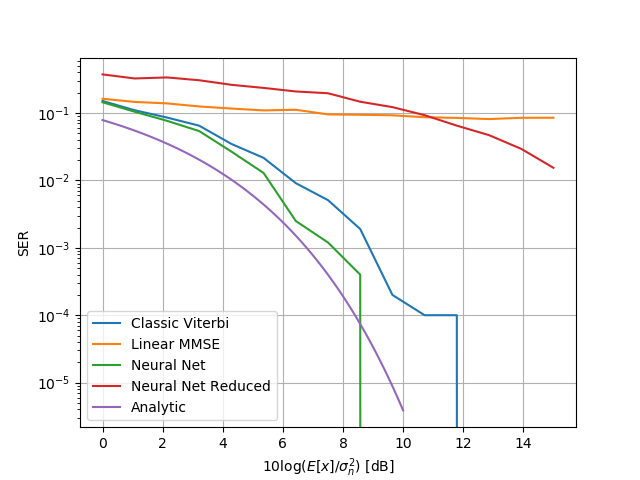
\includegraphics[width=\textwidth,height = 10cm]{results/lti_8_reduced}
		  \caption{Detection performance over LTI channel with AWGN. The LTI channel has impulse response  $[.9, 0, .0, .4, .7]$.}
	  \label{fig:LTI performance redundant}
\end{figure}
\begin{figure}[H]
	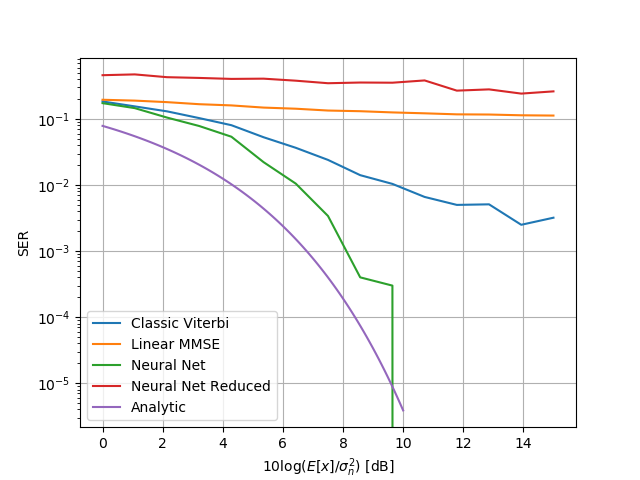
\includegraphics[width=\textwidth,height = 10cm]{results/lti_32_reduced_asymmetric}
		  \caption{Detection performance over LTI channel with AWGN.  The LTI channel has impulse response  $[0.9, 0.7, 0.3, 0.5, 0.1]$.}
	  	  \label{fig:LTI performance}

\end{figure}
\par
We now consider the same LTI channels above but with the receiver quantization, defined in equation \eqref{lti_quantized_channel} and plotted in Figure \ref{fig:Quantized Overlay}, which rounds the received signal to a single decimal place. The upper and lower saturation levels of the quantizer are chosen based on the set of training data such that no received symbols are clipped to the saturation level.
Figures \ref{fig:LTI performance quantized reduced} and \ref{fig:LTI performance quantized} show the results of these simulations. While in both cases, the reduced-state neural network-based equalizer performs poorly, the standard neural-network based equalizer performs well, indicating that this method is capable of learning the distribution function $p(\mathbf{x}|\mathbf{y})$ for non-linear channels. 

\begin{figure}[htp]
	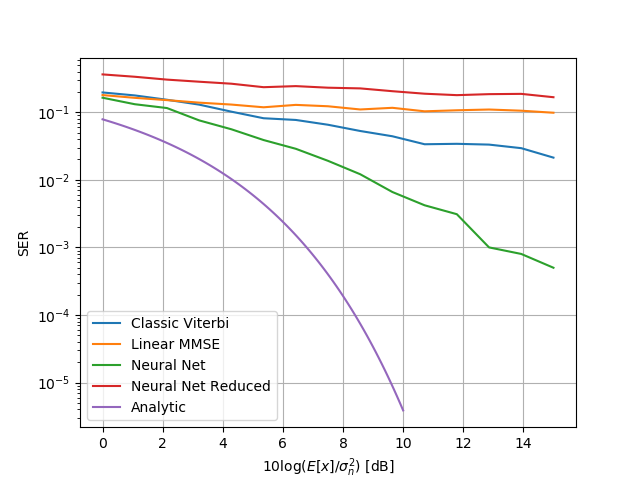
\includegraphics[width=\textwidth,height = 10cm]{results/lti_8_reduced_quantized}
		  \caption{Detection performance over quantized, LTI channel with AWGN. The LTI channel has impulse response  $[.9, 0, 0, .4, .7]$. }
	  \label{fig:LTI performance quantized reduced}
\end{figure}

\begin{figure}[H]
	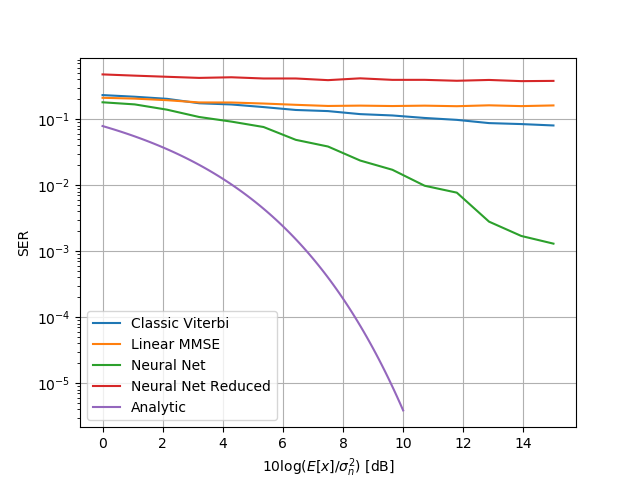
\includegraphics[width=\textwidth,height = 10cm]{results/lti_32_reduced_asymmetric_quantized}
		  \caption{Detection performance over quantized LTI channel with AWGN.  The LTI channel has impulse response  $[0.9, 0.7, 0.3, 0.5, 0.1]$.}
	  \label{fig:LTI performance quantized}
\end{figure}

%Last, we evaluate the LTI channels with quantization and the additional channel randomness described in equation \eqref{lti_quantized_channel}. 


\section{Conclusion}
In this work, a framework is developed in order to define the class of channels to which the channel estimation techniques shown in the work from \cite{shlezinger2019viterbinet} can be applied. Our framework shows that the methods in \cite{shlezinger2019viterbinet} can be used in order to learn channels with addition types of randomness. The framework also outlines a method for complexity reductions in the resulting Viterbi Algorithm. 
 In the simulation work, the results of \cite{shlezinger2019viterbinet} are extended to show that the neural network-based equalizer is capable of channel estimation for  non-linear channels and may be a viable method for estimating channels in the molecular communications domain. 
 \par 
 In future work, this general framework should be explored in related detection algorithms such as those used in \cite{shlezinger2020datadriven}. Further simulation should also be performed for evaluating the detection performance over channels with other non-linearities and random behavior. 

